\documentclass{article}
\usepackage{multicol}
\usepackage{graphicx}
\graphicspath{ {images/} }

\begin{document}
    \section*{CLASE 1 - Taller Base de Datos 272}
    \begin{multicols}{2}
        \subsection{Panorama general de las bases de datos relacionales}
        \underline{\textbf{Datos :}}
        los datos son entidades relaticas a personas, objetos, lugares, y acontecimientos.
        Para ser utiles, los datos deben estar organizados en forma logica y consecuente
        \underline{\textbf{Estructura de Datos :}}
        Las estructuras de datos son técnicas para lograr la organización lógica de datos en
        un sistema de computación.\\
        \underline{\textbf{Informacion :}}
        Los datos organizados y procesados de manera significativa que facilitan su
        interpretación y la toma de decisiones se denominan información.
        La información es subjetiva y su significado depende de la interpretación
        del receptor.\\
        \underline{\textbf{Base de datos :}}
        Es una coleccion de archivos, lógicamente interrelacionados y estructurados,
        independientemente de los programas que lo utilizan y por consiguiente de los 
        usuarios.\\

        \textbf{Participantes en el contexto de las bases de datos}
        \begin{itemize}
            \item El administrados de la base de datos.
            \item Los diseñadores de la base de datos.
            \item Los programadores de aplicaciones.
            \item Los usuarios.
        \end{itemize}
        \subsection{Evolucion Base de Datos}
        \subsubsection{Primera Generacion :}
        \begin{itemize}
            \item Su raiz es en la decada 60, proyecto lunar APOLLO.
            \item Mediados de los 60 aparecio IDS(Integrated Data Store) de general Electric,IMS(Integrated Management System) de IBM.
            \item 1967 se cero la organización DBGT(Data Base Task Group) para especiicar un estándar dando orígen a CODASYL o DBTG.
        \end{itemize}

        \subsubsection{Segunda Generacion}
        \begin{itemize}
            \item Codd de IMB definiio el modelo de datos relacional, abriendose paso a las DB comerciales.
            \item Proyecyo system R de IBM condujo a desarrollar SQL y se implementarion productos como: DB2,SQL/DB, ORACLE.
            \item Todo esto dio paso al desarrollo de los SGBD(DBMS) relacionales.
            \item Sustemas orientados a los datos, los datos se organizan y mantienen en un conjunto estruturado que no esta diseñado para la aplicacion concreta.
            \item Satisface las necesidades de toda la organizacion.
            \item Datos independientes de los tratamientos.
            \item Redundancia controlada.
            \item Datos interrelacionados.
            \item Estructura de datos intregrada y centralizda.
        \end{itemize}


        \subsubsection{Tercera Generacion}
        \begin{itemize}
            \item Creciente complejidad de los datos y las aplicaciones que los tratan.
            \item OODBMS - Base de Datos Orientadas a Objetos.
            \item ORDBMS - Bases de datos objeto relacionales.
            \item Amplian la expresividad pero se alejan del modelo relacional original.            
        \end{itemize}
        \subsubsection{Ventajas de las Bases de datos}
        \begin{itemize}
            \item Independencia de datos (tratamiento)/
            \item Coherencia : No existe redundancia .
            \item Disponibilidad : los datos no son propiedad del usuarios.
            \item Mayor accesibilidad de los datos .
            \item Mayor Valor informativo.
            \item Mejora y mas normalizada documentacion .
            \item Reduccion de espacio de alamacenamiento.
            \item Mayor nivel de concurrencia
            \item Servicios de copia de seguridad y recuperacion.
        \end{itemize}

        \subsubsection{Inconvenientes de las Bases de Datos}
        \begin{itemize}
            \item Instalacion costosa tanto en equipo fisico como logico
            \item Personal especializado para una administracion y correcta
            \item Mayor impacto de fallos
            \item Desfase entre teoria y practica
            \item implantacion larga y dificil
        \end{itemize}
        \subsubsection{Niveles de ABstraccion de las BDS}
        \begin{itemize}
            \item Estructura Logica : Datos Relacionales, restricciones de uso(Derecho a insertar, borrar) de cada usuario.
            \item Nivel Conceptual : Todos los datos interrelaciones, restricciones de integridad, y conficendialidad. independiente del equipo o usuario.
            \item Nivel Fisico : Asignacion de espacios de almacenamiento estrategias de almacenamiento y caminos de accseso.
         \end{itemize}

         \subsubsection{El SGBD}
          Conjuntos de programas, procedimientos y lenguajes que suministra medios a los usuarios, analistas,programadores o administradores para describir,
          recuperar y manipular los datos manteniendo la integridad, confidencialida dy seguridad.
         \subsubsection{Sistema de administracion de Base de datos }
         El objetivo es eficiente para extraer, almacenar, y manipular informacion de la base de datos.
         Todas las peticiones de acceso a la base de datos, se manejan centralizadamente por medio del DBMS, por lo que este paquete funciona como interfaz entre los usuarios y la base de datos.
         \subsubsection{Funciones de un SGBD}
            \begin{itemize}
                \item Definicion : Permite especificar los elementos de datos, estructura y las relaciones que existen entre ellos,las reglas de integridad semantica, controles a efectuar antes de autorizar el acceso a la DB.
                \item Manipulacion : permite a los usuarios buscar, añadir suprimir o modificar los datos siempre de acuerdo con las espedificaciones y normas de seguridad especificadas.
                \item Utilizacion : Esta funcion reune todas las interfaces que necesitan los diferentes usuarios para utilizar la base,ademas de proporcionar un conjunto de procedimientos para el administrador.
            \end{itemize}
         \subsubsection{Instrucciones  SQL -DDL}
         Empleados para \textbf{Crear, Modificar o Borrar} objetos en una base de datos como tablas, vistas, esquemas, dominios,activadores, y almacenar procedimientos.
         \begin{itemize}
            \item CREATE : La consulta CREATE se utiliza para crear una base de datos u objetos como tablas, vistas, procedimientos almacenados, etc.
            \item ALTER : El comando ALTER en SQL DDL se usa para modificar la estructura de una tabla ya existente.
            \item TRUNCATE : El comando TRUNCATE en SQL DDL se usa para eliminar todos los registros de una tabla.
         \end{itemize}
         \subsubsection{Instrucciones SQL -  DML}
         \begin{itemize}
            \item SELECT : Se utiliza para recuperar datos de la base de datos.
            \item INSERT :Se utiliza para insertar datos en una tabla
            \item UPDATE :Se utiliza para actualizar los datos existentes dentro de una tabla
            \item DELTE :Se utiliza para eliminar registros de una tabla de base de datos.
         \end{itemize}
        \end{multicols}
         \newpage
         \section{CLASE 2 - Taller Base de Datos 272}
         \begin{multicols}{2}
            \subsection{Instrucciones SQL-DML}
                Empleadas para \textbf{SELECCIONAR, INSERTAR, ACTUALIZAR,BORRAR} registros en una tabla de una base de datos.
                    \begin{itemize}
                        \item SELECT : 
                        \item INSERT  : insertar registro a una tabla.
                        \item UPDATE : modificar informacion almacenada.
                        \item DELTE : eliminar registros en el interior de la tabla.
                        \item MERGE : mesclar 2 o 3 tablas si llegasen a tener elememtos comunes y genera una nueva tabla.
                    \end{itemize}
            \subsection{Instrucciones SQL-DDL}
                Empleadas para \textbf{CREAR, MODIFICAR, BORRAR} objetos en una base de datos como tablas, vistas, esquemas, dominios, activadores, y almacenar procedimientos, usuarios.
                    \begin{itemize}
                        \item CREATE : crea estructura.
                        \item ALTER  : modificar una tabla o estructura.
                        \item DROP : crear,modificar,borrar.
                        \item RENAME : renombrar
                        \item TRUNCATE : eliminar fisicamente una tabla.
                    \end{itemize}
            \subsection{Instrucciones SQL-DCL}
                    Permite crear y gestionar permisso y accesos a los datos
                    \begin{itemize}
                        \item GRANT : otorgar permisos
                        \item REVOKE  : quitar permisos
                    \end{itemize}

            \subsection{Ejercisios}
                    Se usaran 3 comandos
                    \begin{itemize}
                        \item CREATE
                        \item INSERT
                        \item SELECT
                    \end{itemize}
                    Entidades y atributos a usar :\\
                    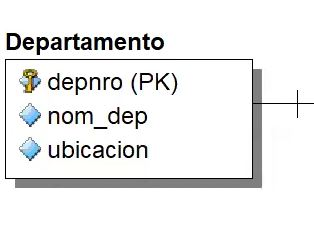
\includegraphics[width=4cm]{/2022-2/272/Apuntes/img/Img_1.JPG}\\
                    Entidad Departamento.\\
                    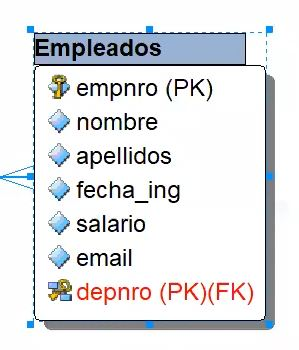
\includegraphics[width=4cm]{/2022-2/272/Apuntes/img/Img_2.JPG}\\
                    Entidad Empleados\\ 
                    \newpage                       
                    \subsection{Tipos de datos}
                    \begin{itemize}
                        \item CHAR(N)
                        \item VARCHAR2(N)
                        \item NUMBER(P,S) p = cantida de digitos y s = cantida de decimales
                        \item DATE
                    \end{itemize} 
                    
                                    
            \subsection{CREATE}
            
                \begin{tabular}{| c |}\hline            
                    
                    create table DEPARTAMENTOS(\\
                    NombreColumna tipo \\ 
                    ,NombreColumna tipoDeDatos...\\
                    ,definicion de clave primaria \\
                    ,definicion de clave foranea);\\ \hline
                    Creando tabla DEPARTAMENTO\\ \hline
                    create table\\ 
            DEPARTAMENTOS(\\
             depnro number,\\ 
            nomdep varchar2(50) not null, \\ 
            ciudad varchar2(50) not null, \\ 
            PRYMARY KEY  depnro );\\ \hline
            

                    \end{tabular}
            
            \subsection{INSERT}
            \begin{tabular}{| c |}\hline 
                INTO tabla(\\
                campo1,campo2,...,campo n)\\ \hline
                Insertando departamento\\ \hline
                insert into departamentos(\\
                depnro,nomdep,ciudad)values\\
                 (1,'Marketing' \\
                 ,'Santa Cruz de la Sierra');\\ \hline
                \end{tabular}
            \subsection{SELECT}
            \begin{tabular}{| c |}\hline 
                selecto*from nombretabla\\ \hline
                Mostrar toda la tabla empleados\\ \hline
                select * from empleados; \\ \hline
                Mostrar algunos(nombre.apellido,cargo) datos de la tabla \\ \hline
                select nomemp,apeemp,cargo from empleados;\\ \hline
                Mostrar solo los datos que no se repiten en la tabla\\ \hline
                select disctinct cargo from empleados;\\ \hline
            \end{tabular}
         \end{multicols}

        
        

\end{document}